\documentclass[11pt,a4paper]{article}

\usepackage{indentfirst}
\usepackage{amssymb}
\usepackage{subcaption}
\usepackage{graphicx}
\usepackage{longtable}
\usepackage{fancyhdr}
\usepackage{xeCJK}
\usepackage{amsmath}
\usepackage{amssymb}
\usepackage{ulem}
\usepackage{xcolor}
\usepackage{fancyvrb}
\usepackage{listings}
\usepackage{soul}
\usepackage{hyperref}
	\lstdefinestyle{C}{
   		language=C, 
   		basicstyle=\ttfamily\bfseries,
    	numbers=left, 
    	numbersep=5pt,
    	tabsize=4,
    	frame=single,
   	 	commentstyle=\itshape\color{brown},
    	keywordstyle=\bfseries\color{blue},
   	 	deletekeywords={define},
    	morekeywords={NULL,bool}
	}	

\setCJKmainfont{Noto Sans Mono CJK TC}
 
\voffset -20pt
\textwidth 410pt
\textheight 650pt
\oddsidemargin 20pt
\newcommand{\XOR}{\otimes}
\linespread{1.2}\selectfont
\graphicspath{{images/}}

\pagestyle{fancy}
\lhead{國立宜蘭高中 111 學年度資訊學科能力競賽}

\begin{document}

\begin{center}
\section*{F. 波動的麥穗}
\end{center}

\section*{Description}

傳說蘇格拉底曾經帶領幾個弟子來到一個麥穗田邊,請他們去摘下一個最高最好的麥穗。
不過他們必須頭也不回地沿著直線前進,且只有一次的摘取機會。
這個故事逐漸演變成數學裡的最優停止問題(Optimal Stopping Problem),並且找到了最佳解 —— $37\%$ 法則。
也就是記住前 $37\%$ 中最高最好的麥穗,接著在後 $63\%$ 裡頭遇到的第一個更好的麥穗即是最佳選擇。

某晚小晨在睡夢中偶遇了蘇格拉底,最近因為股市起起落落而心情大受影響的小晨,忍不住跟蘇格拉底抱怨一番。
為了鼓勵小晨繼續努力前進,蘇格拉底又講述了一個麥穗的故事。
不同於先前的版本,這次蘇格拉底希望小晨去尋找一些高度波動的麥穗,就好像那高高低低的股價一般。
蘇格拉底說到

\vspace{0.6cm}
「小晨啊,你看看眼前的 $N$ 個麥穗,每個都有不同的高度 $h_i$ 跟價值 $v_i$。
不如你就去尋找一些麥穗,使得你依序選定的這些麥穗高度是波動的,且價值總和最高。
相信這一定會對你的人生有所幫助吶!」
\vspace{0.6cm}

更確切地說,若 $h_1, h_2, \cdots, h_k$ 依序是小晨選定的麥穗高度,則這些高度必須滿足波動形式:
$$
	\left(h_{j-1} < h_j > h_{j+1}\right) \vee 
	\left(h_{j-1} > h_j < h_{j+1}\right)
	,\quad \forall j \in [2, k-1]
$$
也就是這些選定的麥穗一字排開的話,高度會呈現一高一低的鋸齒狀。

小晨醒來後,急忙拿著這 $N$ 筆麥穗的資料翻來覆去,嘗試尋找最佳的選擇。
然而由於麥穗實在是太多了,小晨怎麼樣也無法好好確認所有的可能性。
請你幫助小晨,找到最佳選擇下,他能夠拿到多少價值總和的麥穗,讓他的人生可以稍微減少一點悲慘。

\section*{Input}

第一行包含一個正整數 $N$,代表麥穗的數量。

接下來 $N$ 行,每行有二個整數 $h_i, v_i$,分別代表第 $i$ 個麥穗的高度與價值。

各變數範圍限制如下:
\begin{itemize}
    \item $1 \le N \le 2\times 10^5$
    \item $-10^9 \le h_i, v_i \le 10^9$
\end{itemize}

\section*{Output}

請輸出一個整數,代表最高可能的價值總和。

\section*{Sample 1}
\begin{longtable}[!h]{|p{0.5\textwidth}|p{0.5\textwidth}|}
\hline
\textbf {Input}	& \textbf {Output} \\
\hline
\parbox[t]{0.5\textwidth} % sample 1
{ \tt
% input
10 \\
2 7 \\
3 5 \\
6 1 \\
5 3 \\
7 2 \\
1 8 \\
3 9 \\
6 2 \\
4 1 \\
5 3 \\
} &
\parbox[t]{0.5\textwidth}
{ \tt
%output
30 \\
} \\
\hline
\end{longtable}

\section*{Sample 2}
\begin{longtable}[!h]{|p{0.5\textwidth}|p{0.5\textwidth}|}
\hline
\textbf {Input}	& \textbf {Output} \\
\hline
\parbox[t]{0.5\textwidth} % sample 2
{ \tt
% input
6 \\
1 -5 \\
2 4 \\
2 -2 \\
2 3 \\
1 -1 \\
2 2 \\
} &
\parbox[t]{0.5\textwidth}
{ \tt
%output
5 \\
} \\
\hline
\end{longtable}

\section*{Sample 3}
\begin{longtable}[!h]{|p{0.5\textwidth}|p{0.5\textwidth}|}
\hline
\textbf {Input}	& \textbf {Output} \\
\hline
\parbox[t]{0.5\textwidth} % sample 3
{ \tt
% input
1 \\
-7777 -9999 \\
} &
\parbox[t]{0.5\textwidth}
{ \tt
%output
0 \\
} \\
\hline
\end{longtable}

\section*{配分}

在一個子任務的「測試資料範圍」的敘述中,如果存在沒有提到範圍的變數,則此變數的範圍為 Input 所描述的範圍。

\begin{center}
 \begin{tabular}{||c c c||} 
 \hline
 子任務編號 & 子任務配分 & 測試資料範圍 \\  
 \hline\hline
 1 & 0\% & 範例測資 \\ 
 \hline
 2 & 8\% & $1 \le N \le 20$ \\
 \hline
 3 & 13\% & $1 \le h_i \le 2$ \\
 \hline
 4 & 28\% & $1 \le N \le 1000$ \\
 \hline
 5 & 32\% & $1 \le h_i \le 2\times 10^5$ \\
 \hline
 6 & 19\% & 無額外限制 \\
 \hline
\end{tabular}
\end{center}

\section*{Hint}
下圖為範例一的麥穗及最佳選擇。

$X$ 軸為節點選擇順序,$Y$ 軸代表高度,旁邊的數字代表價值。
紅色節點為選定的麥穗,其連線呈現波動狀。
\begin{center}
	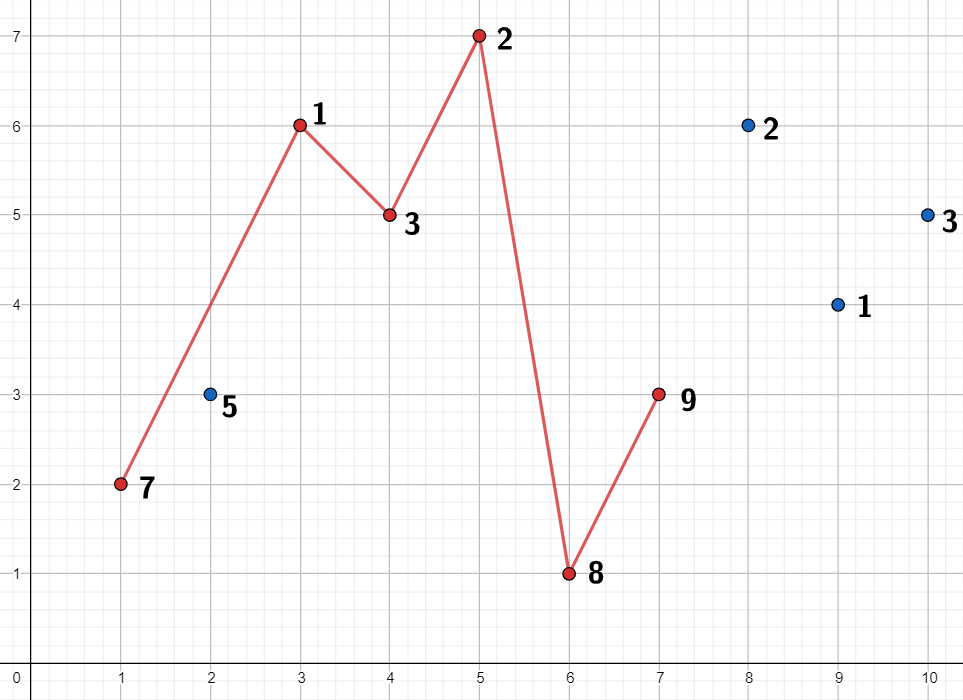
\includegraphics[width=10cm]{sample1.png}
\end{center}

注意到範例三中,不拿取任何麥穗亦是一種選擇。

\end{document}
